\scanpage{27}
\mspage{25}
Voici les résultats positifs que j'ai vérifiés dans la direction des assertions précédentes:

a) Si $S$ est de caractéristique nulle, les assertions 1º et 3º (sous la forme précisée par l'introduction du schéma en groupes $G(A)$) sont vraies.

b) Sans restrictions sur $S$, il est vrai que $G(A)$ n'a pas d'automorphismes infinitésimaux, donc si pour deux relèvements infinitésimaux \inserted{donnés} $B,B'$ de $A$, $G(B)$ et $G(B')$\deleted{\unsure{,}} sont isomorphes, l'isomorphisme\deleted{s} entre eux est unique. Donc si l'\deleted{assertion} \inserted{hypothèse} précédente est \deleted{vrai} \inserted{\unsure{vérifiée|vérifié}}, quels que soient les relèvements infinitésimaux de $A$ au dessus d'un ouvert $U$ de la base $S$, alors les $G(B)$ définissent effectivement un cristal \inserted{en groupes} sur $S$, à fortiori les $H(B)$ définissent un cristal de modules, et $G(A)$ et $H^1_{\operatorname{DR}}(A/S)$ sont\deleted{\unsure{s}} munis de stratifications absolues canoniques, fonctorielle\inserted{s}, d'ailleurs en $A$ satisfaisant aux conditions envisagées, et compatible avec tout changement de base qui invarie notre hypothèse sur $A$.
\margin{faux}

c) Les assertions 1º à 3º (sous la forme précisée par $G(A)$) sont vraies pour les relèvements infinitésimaux \uline{d'ordre} 1, ou tout au moins lorsque $T$ est de la forme $D(\underline{J})$, schémas des nombres duaux défini par un $\underline{J}$ quasi-cohérent.
\margin{\figure{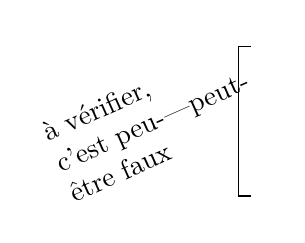
\begin{tikzpicture}
\draw (2.1,0) -- (1.95,0) -- (1.95,1.9) -- (2.1,1.9);
\node[align=left,rotate=24] at (0.85,0.95) {à vérifier,\\c'est \unsure{peu-|peut-}\\\uline{être faux}};
\end{tikzpicture}}}

2.7. Arrivé à ce point de mes brillantes conjectures, je m'aperçois avec consternation qu'elles sont fausses telles quelles, malgré les indications concordantes militant en leur faveur. De façon précise, soit $k$ un corps de caractéristique \deleted{nulle} $p>0$. Je dis qu'\uline{il n'est pas possible}, \uline{pour tout} $k$-\uline{schéma} $S$ \uline{de type fini}, \uline{de dimension} $\le\deleted{1}\inserted{0}$, \uline{avec} $S_{\text{rég}}$ \uline{régulier}, \uline{et tout schéma elliptique} \uline{$A$ sur} $S$, \uline{de mettre sur} $H^1_{\operatorname{DR}}(A/S)$ \uline{une stratification relativement à} $k$, \uline{qui soit fonctorielle en} $A$ \uline{et compatible avec les changements de base}. L'ennui, comme d'habitude, provient des courbes elliptiques de Hasse nul. Appliquant en effet les deux fonctorialités postulées, on trouve que l'homomorphisme ``frobenius'' qui va de $M^{(p)}$ dans $M$ ($M=H^1_{\operatorname{DR}}(A/S)$) serait compatible avec la stratification. Si alors $s\in S$ est un point correspondant à un $A_s$ de Hasse nul, i.e. tel que frobenius sur $H^1_{\operatorname{DR}}(A_s)$ soit de carré nul, on en conclurait aisément, grimpant sur les voisinages infinitésimaux de $s$, que la même propriété serait vraie aux points voisins de $s$, ce qui est évidemment faux p.ex. pour la famille modulaire.
\margin{\figure{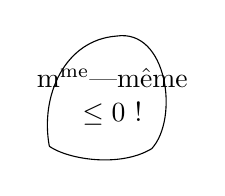
\begin{tikzpicture}
\draw (0,0.15) .. controls (-0.12,0.8) and (0.2,1.5) .. (0.85,1.55) .. controls (1.5,1.65) and (1.65,0.5) .. (1.3,0.12) .. controls (0.9,-0.12) and (0.25,-0.02) .. (0,0.15);
\node[align=center] at (0.8,0.78) {\unsure{m\textsuperscript{me}|même}\\$\le0$ !};
\end{tikzpicture}}}
\margin{26}
